\section{Background}
\label{sec:back}
In this section, we will review the MapReduce programming
model and detail the salient features of Phoenix, 
an implementation of MapReduce for multicore.
%Then the limitation of Phoenix in the aspect of performance is analyzed.
%讨论Phoenix的局限与不足

\subsection{MapReduce Programing Model}
Inspired  by funnctional languages, the MapReduce programming model is proposed for data intensive computation in cluster environment.
Its simple programming interface requires programmer to  define only two primitives: map and reduce.
The map function is applied on the input data and produces a set of intermediate key-value pairs.
The reduce function is applied on all intermediate pairs and  groups them with the same key to a single key-value pair. 
In order to save networking bandwidth and reduce memory consumption, the combine function, an optional operation, can aggregate the key-value pairs locally in Map phase.


The charm of MapReduce is that, for applications that can adapt, it hides all the concurrency details from  programmer. 
For example, one can count the number of occurrences for each word in a text file. 
The map function emits a $\langle word, 1\rangle$ pair for each word in document, and the reduce function counts all occurrences of a word as the output. 
The combine function is similar to the reduce function, but only processes a partial set of key-value pairs in Map phase.


\subsection{Phoenix}
Phoenix is an implementation of MapReduce for multicore  and multiprocessor systems using Pthreads.
It shows MapReduce model is a promising model, and the applications written with MapReduce have competitive scalability and performance in comparison to those written with Pthreads\cite{ranger2007phoenix};
Phoenix stores the intermediate key-value pairs produced 
by the map workers in a global matrix (Figure \ref{fig:phoenix:intermediate}). 
Each map and reduce workers can write or read this global matrix. 
%Concurrent map workers can touch the same area without synchronous controls.
When map and reduce workers operate the matrix concurrently,
two strategies must be carried out to avoid lock contention costs.
\begin{itemize}
	\item Each row of the matrix is exclusively used by a map worker, and each column of the matrix is exclusively used by a reduce worker. 
%	\item There is a barrier between the Map and Reduce phase. After all map workers have been completed, the reduce workers begin to compute. 
	\item There is a barrier between the Map and Reduce phase. Only when all map workers have been completed do the reduce workers begin to compute. 
\end{itemize}

\begin{figure}[!h!t]  
    \centering
    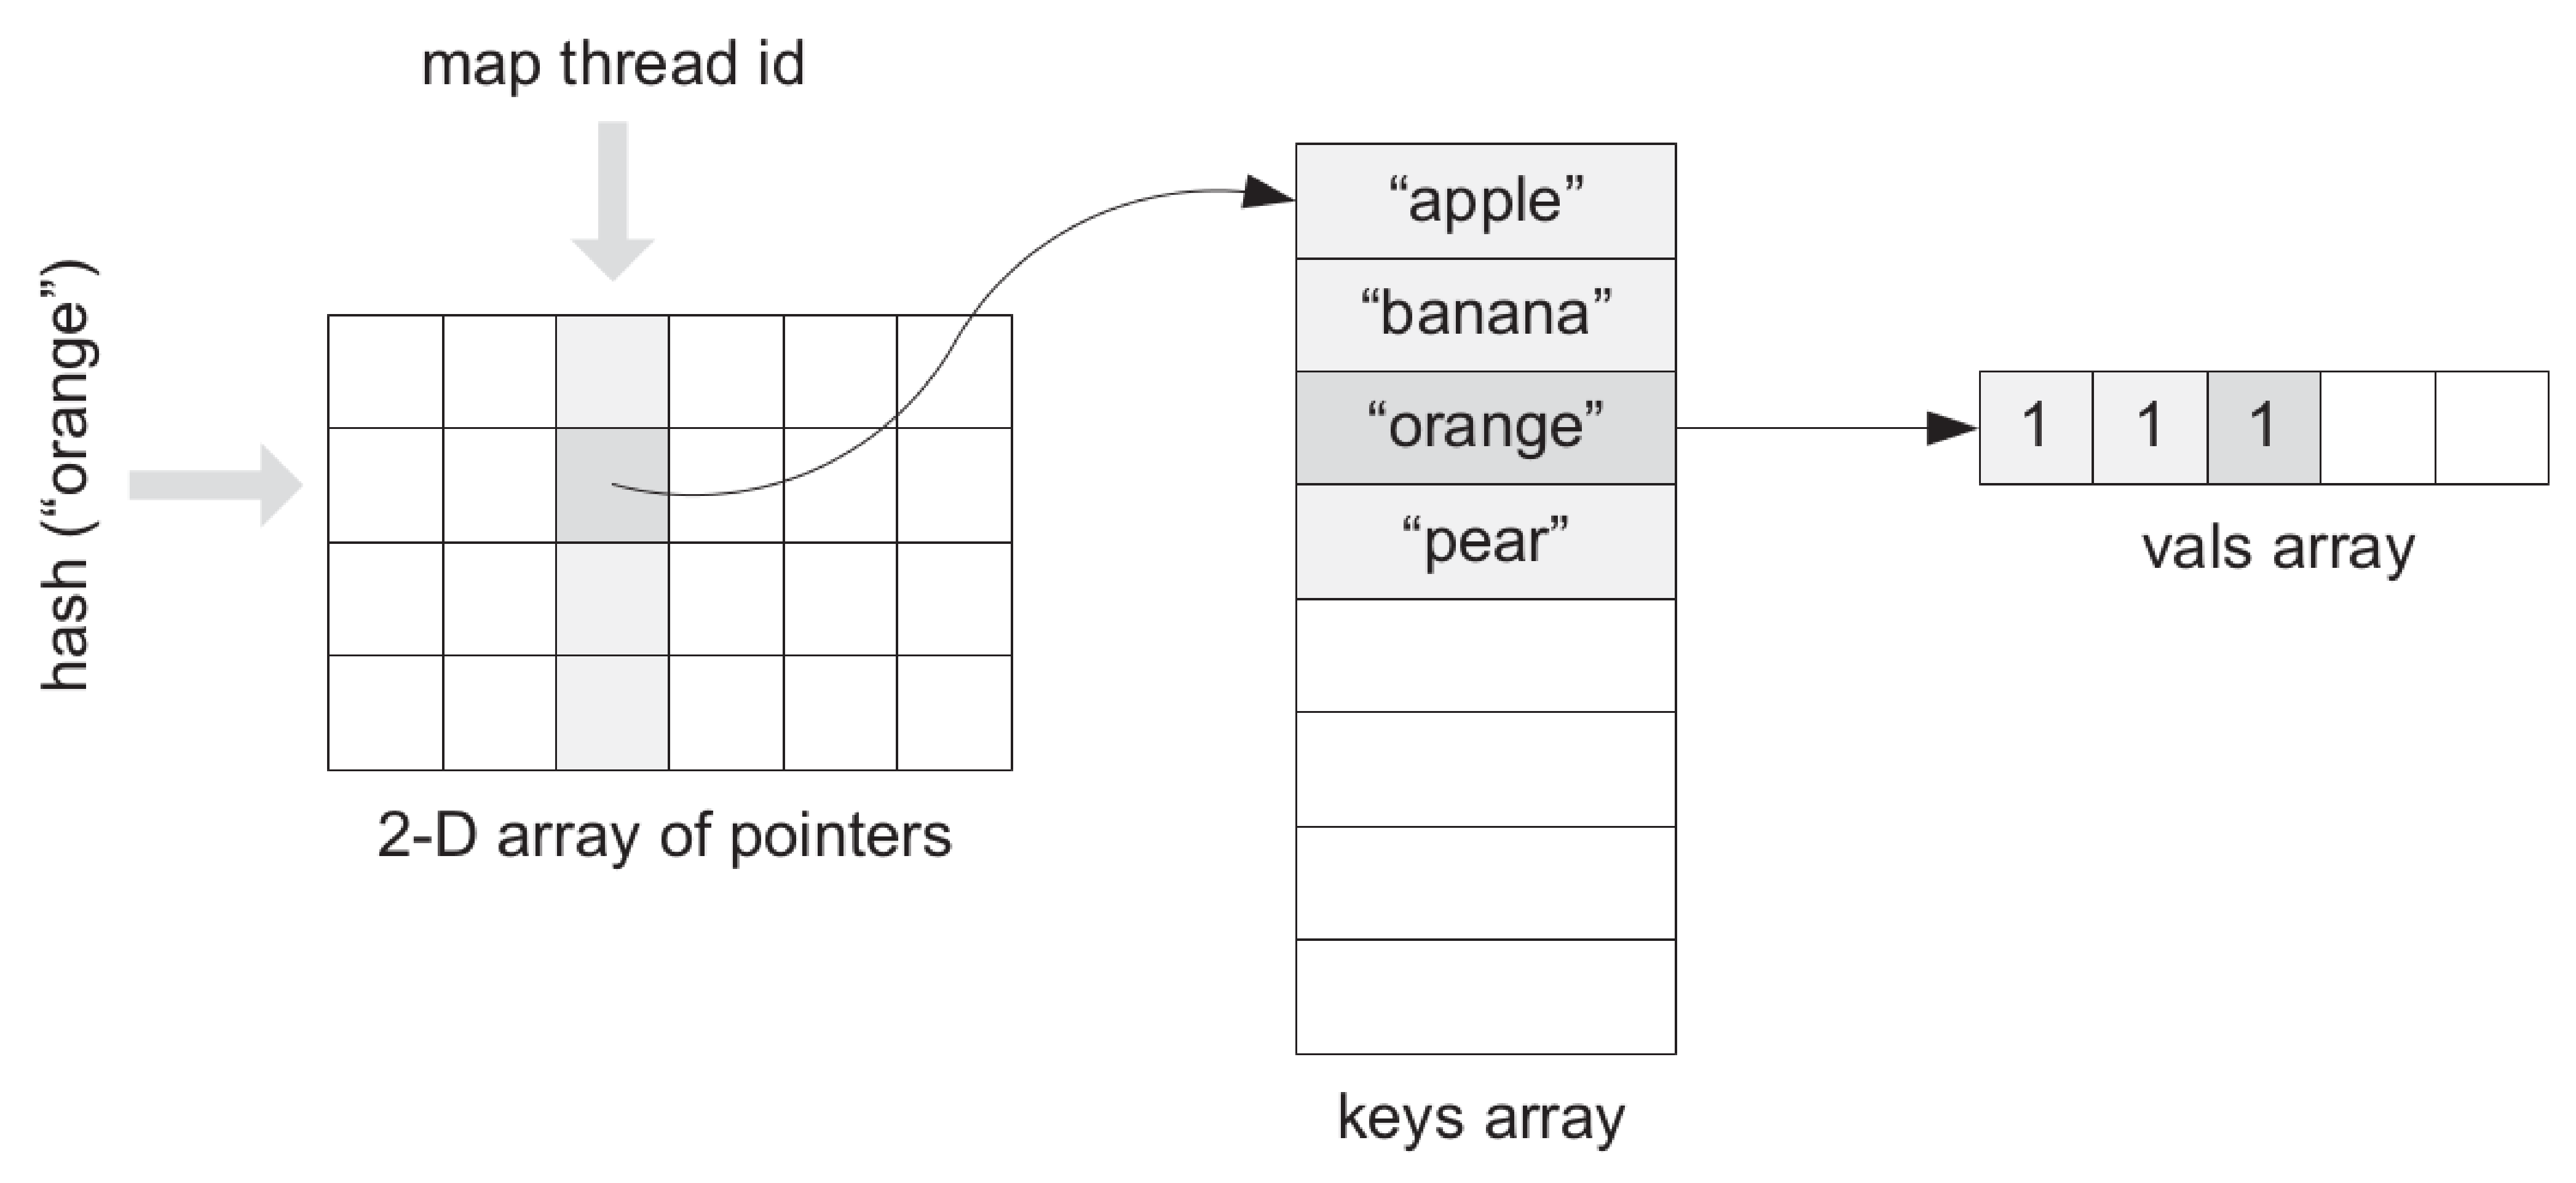
\includegraphics[width=0.45\textwidth]{eps/phoenix_intermediate.eps}
    \caption{Phoenix intermediate struct}
    \label{fig:phoenix:intermediate}
\end{figure}

By adopting above strategies, applications programming with Phoenix can effectively reduce lock contention costs. 
However, these strategies limit the performance of Phoenix, which will be described in next Section. 

\section{Analysis of Phoenix}
%Phoenix demonstrates tha applications that fit the MapReduce model can perform competitively with parallel code using Pthreads.

%Though Phoenix has demonstrated promising feasibility when running applications on multicore, it has limitations in terms of scalability and performance due to its manners of design and implementation.
In this section, we first evaluate Phoenix built with a scalable memory allocator.
Then we will analyze the important roadblocks that limit scalability and performance of the Phoenix runtime on shared-memory systems.



\subsection{Scalability}
%We first evaluate the scalability of Phoenix built with jemalloc, a good scalable memory allocator, and than we measure the scalability of \myds to demonstrate the effectivity of \myds.
Since there are many heap objects shared among threads in Phoenix, it is sensitive to memory allocator\cite{yoo2009phoenix2}.
The memory allocator in glibc (i.e.,  ptmalloc\cite{gloger1997ptmalloc}) does not scale on multicore system, while jemalloc\cite{evans2006jemalloc} can provide improved performance and scalability. 
Therefore, we evaluate the scalability of Phoenix built with jemalloc, denoted as \codet{Phoenix-jemalloc}.

\begin{figure}[!h!t]  
	\centering
	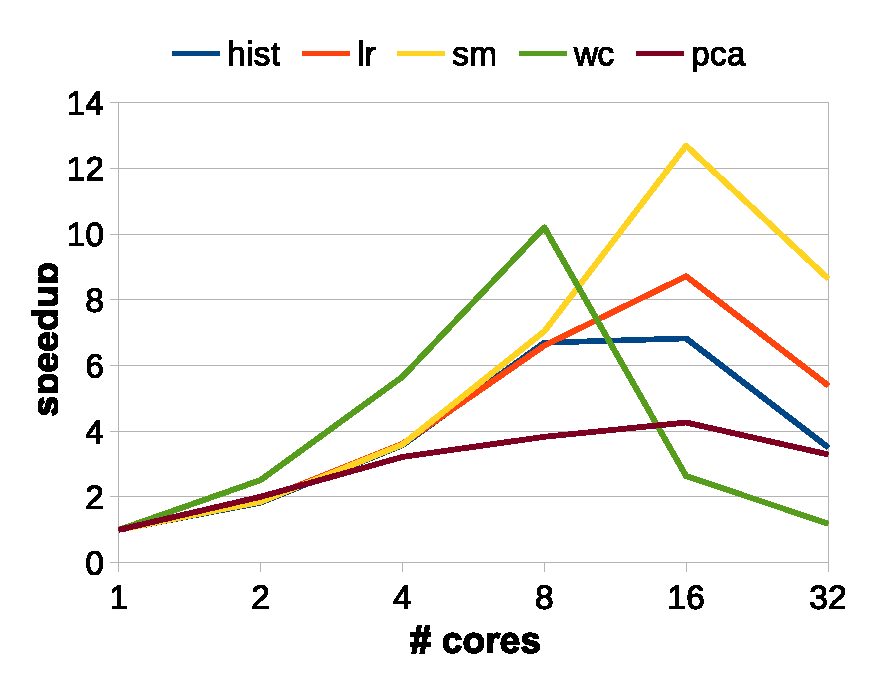
\includegraphics[width=0.45\textwidth]{eps/phoenix_speedup_jemalloc.eps}
	\caption{speedup of Phoenix-jemalloc}
	\label{fig:phoenix:speedup:jemalloc}
\end{figure}

%For linear\_regression (lr) and string\_match (sm),  using 16 or more  cores leads to speedup degradation.

Figure \ref{fig:phoenix:speedup:jemalloc} illustrates the speedup of Phoenix built with jemalloc.
We observe that applications scale well when the core count increases from 1 to 8.
However, when the core count increases from 8 to 16 to 32, the speedup sharply degrades for \codet{wc} and from 16 to 32 cores for the other applications.
The results indicate that in spite of utilizing the scalable memory allocator, Phoenix can not scale up to 16 cores.

In order to analyze the limited scalability behavior, Linux perf is exploited to collect execution time information of hot function. 
We note that the map function is the hottest function with less cores, while \lock will become the hottest function with more cores.
\lock is a type of spinlock which is caused by the contention on the shared structure in Linux kernel.
In order to specially explore the impact of spinlock in Phoenix, we collect the execution time percent of \lock on each benchmark from 1 to 32 cores by Linux perf.

\begin{figure}[!h!t]  
	\centering
	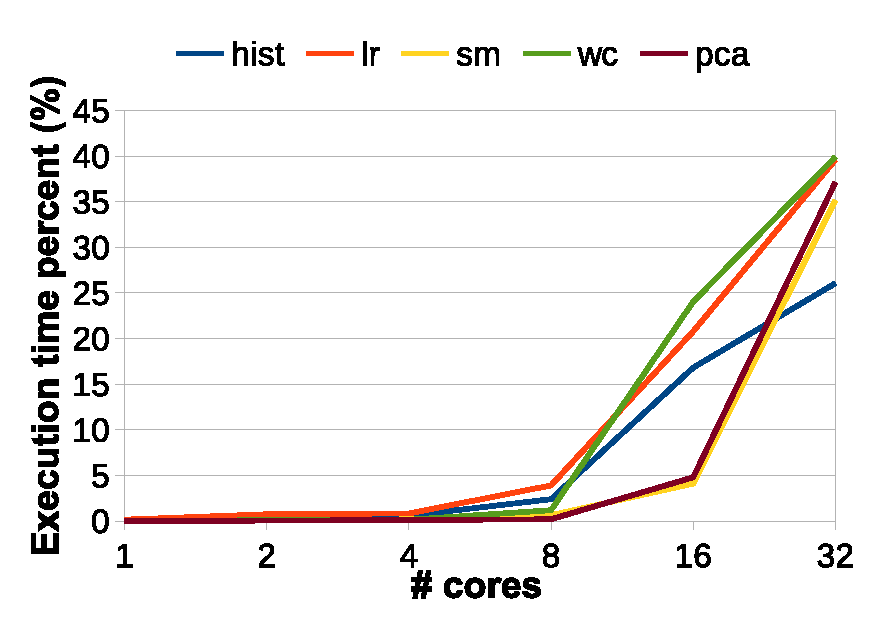
\includegraphics[width=0.45\textwidth]{eps/phoenix_spinlock_jemalloc.eps}
	\caption{\lock percent of applications in Phoenix}
	\label{fig:phoenix:spinlock:jemalloc}
\end{figure}

As the result shows in Figure\ref{fig:phoenix:spinlock:jemalloc}, the cost of spinlock increases quickly as the cores number cross a specific value (i.e., 8).
%Specially, for hist with 16 and 32 cores, \_\_ticket\_spin\_lock is the function that has largest execution time percents of 40.15\%  and 71.25\%, respectively. 
Specially, for \codet{wc} 16 and 32 cores, \lock (\ie spinlock) is the function that has largest execution time percents of \redt{24.04\%} and \redt{39.91\%}, respectively. 
Experiment results demonstrate that Phoenix suffers from serious lock contention when the cores number exceeds 8. 
That means most of execution time will be used for waiting but not actual computation.

%Phoenix performs well with less cores, it can not scale up 16 cores for all applications. 
%Actually, when cores number exceed 8, the speedup of \codet{wc} and \codet{hist} on Phoenix begin degrading. 

%Phoenix performs well with no more than 16 cores.
%However, when core number exceed 16, .
%For lr and sm, the speedup is degraded when cores is greater than 16.


%on \codet{hist}, \codet{wc} and \codet{pca} when the number of core is less than 8.
%As the number of cores increase (from 1 to 8), the performance of Phoenix increase for all cases, i.e., the execution time decreasing. 
%While For 16 to 32 cores, Phoenix performance keep decreasing with the increase of the number of cores.

%The above performance changes can be explained from contending on the shared address space in Linux kernel.
%Therefore, we collect \_\_ticket\_spin\_lock execution time percent information to peek the contention by Linux perf.
%The results as shown in Figure \ref{fig:phoenix:spinlock:jemalloc}, turn out that serious lock contention takes place when increase the number of cores over 8 and as a result execution time will be drastically increased.


%When the number of dependent processes increases above the
%number of cores, serious contending lock takes place,
%and as a result execution time will be drastically increased.
%As the number of threads increases from 32 to 33, 
%there is a significant increase in execution time owing to .

%Overall, increasing cores number results in the growth of speedup for Phoenix at low cores.
%However, 


\subsection{Contention of the single address space}
Phoenix utilizes shared-memory multiple threads to implement parallelism, where all threads of an application share a single address space.
In most widely used operating systems, such as Linux, an address space consists principally of a set of memory mapping regions and a red-back tree is used to store these regions. 
The red-back enables the operating system to find a particular region quickly when a process has have thousands of memory regions \cite{linux}.

Linux provide three address space operations to update and read the memory region: \codet{mmap}, \codet{munmap} and page fault.
The \codet{mmap} operation creates memory mapping regions and adds them to the region red-back tree, while the \codet{munmap} removes the memory regions from the tree.
%munmap removes regions from the tree and invalidates entries in the hardware page table structures. 
Page faults look up the faulting virtual address in the red-back tree to check whether the virtual address is mapped.
To ensure correct behavior when several threads perform \codet{mmap} and page faults concurrently, Linux use a single read/write semaphore per process (\codet{mmap\_sem}) to serialize \codet{mmap} and page faults.
Therefore, threads need to acquire the semaphore in write mode before executing the \codet{mmap} operation, while permitting page faults and the other \codet{mmap} operations.
And page faults will acquire the semaphore in read mode and can proceed with each other in parallel. 

A process can perform only one \codet{mmap} or \codet{munmap} at a time, and these operations will delay page faults. 
In addition, page faults for different virtual addresses run concurrently, but will block other threads from performing \codet{mmap} or \codet{munmap} operations.
As a consequence, the performance of multithread applications will be limited by the serialization. 
The contention is intense when there are large amounts of threads, which will lead to the parallel scalability degradation on the benchmarks.


In Phoenix, benchmarks utilize the mmap() system call to read in input data. 
Once the user passes the pointer of the mmap() region to runtime as an argument, multiple map threads will concurrently cause page faults in the input data when they invoke map functions.
%All of these page faults need to access the unique mmap\_sem semaphore, which is local to a process address space. 
Moreover, there are many \codet{mmap} operations in memory allocator for dynamic memory management in Phoenix, which will lead to contend for the shared address spaces.
As indicated in Figure \ref{fig:phoenix:speedup:jemalloc}, Phoenix can not scale as well as expected, when the cores count exceed a value, adding more cores might scale negatively due to the increased time spent in spinlock.
Experiment call-graph information demonstrates that spinlock is caused by page faults and \codet{mmap} operations.

%Applications will start as many threads as the system's cores in Phoenix.
%Ideally, adding more threads and cores to the runtime would bring about a linear decrease in execution time.
%However, the parallel scalability of Phoenix is not ideal.
%However, Phoenix can not scale as well as expected.

%As more cores were added, the benefit was reversed due to the increased time spent in spinlock.

%That means the time of completing a workload will increase if there are more cores in the system. 

%In order to analyze the limited scalability behavior, Linux perf is exploited to collect execution time information of hot function. 
%We note that the map function is the hottest function with less cores, while \_\_ticket\_spin\_lock will become the hottest function with more cores.
%\_\_ticket\_spin\_lock is a type of spinlock which is caused by the contention on the shared structure in Linux kernel.
%In order to specially explore the impact of spinlock in Phoenix, we collect the execution time percent of \_\_ticket\_spin\_lock on each benchmark from 1 to 32 cores by Linux perf.
%
%As the result shows in Figure\ref{fig:phoenix:spinlock}, the cost of spinlock increases quickly as the cores number cross a specific value (ie. 8).
%Specially, for hist with 16 and 32 cores, \_\_ticket\_spin\_lock is the function that has largest execution time percents of 40.15\%  and 71.25\%, respectively. 
%Experiment results demonstrate that Phoenix suffers from serious lock contention when the cores number exceeds 8. 
%That means most of execution time will be used for waiting but not actual computation.
%Call-graph information shows that \_\_ticket\_spin\_lock is caused by pagefault, which is not scale well on large numbers of cores.

%\begin{figure}[!h!t]  
%	\centering
%	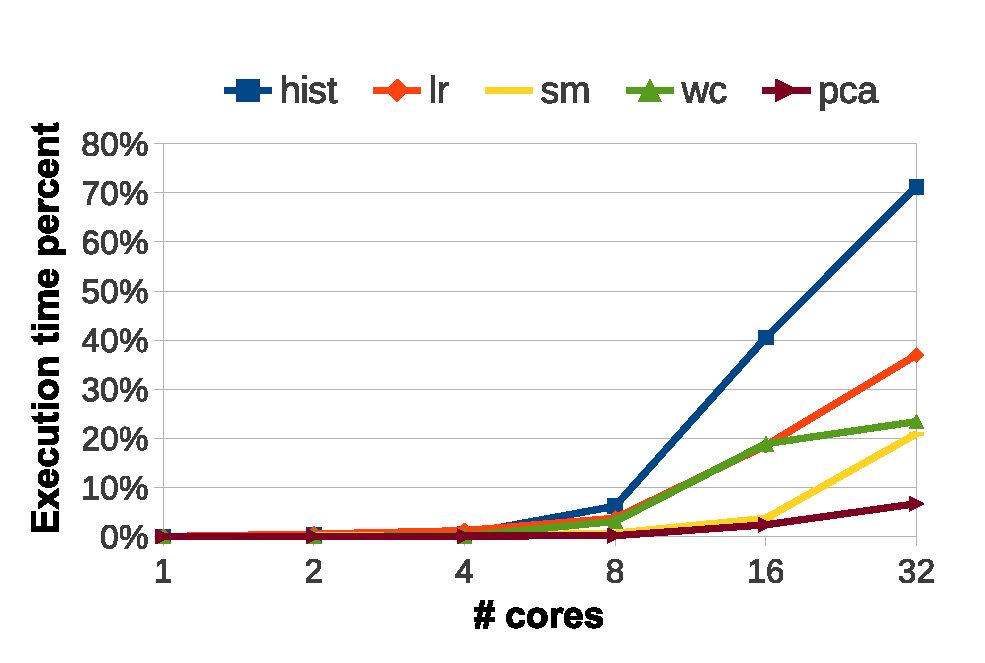
\includegraphics[width=0.45\textwidth]{eps/phoenix_spinlock.eps}
%	\caption{Phoenix ticket\_spin\_lock percent}
%	\label{fig:phoenix:spinlock}
%\end{figure}



%store the memory regions because applications often have thousands of memory regions 

%and a tree enables the operating system to find the region
%containing a particular virtual address quickly
%
%One reason why Linux uses this single semaphore on the address space is that it needs a red-black tree to guarantee $O$(log$n$) lookup time when a process has many mmap memory regions \cite{linux}.




 
%As a result, multiple threads concurrently pagefaults will casue contention to the single semaphore.
 
%The semaphore is a sleep lock and may run into convoying problems,
%where waiting threads may get stuck at the end of the wait queue for a long time \cite{Andi2009lmulticore}.




\subsection{Optimizing opportunities of Phoenix}
In cluster environment, network bandwidth is the key factor for performance since the map and reduce workers, executed in different machines usually, communicate by the network.
However, when processing MapReduce applications in multicore environment, the data structures shared by multiple threads, instead of the network, are the major performance bottlenecks.
% based on applications in Phoenix will naturally suffer from serious contended locks.
%By using a share-memory threads model, multiple threads in Phoenix need to share the process's address space\cite{linux}.
There is a single lock for per shared address space inside the operating system’s virtual memory system, which we have discussed in the previous section. 
As a result, multithreaded applications on many-core processors will naturally suffer from serious contended locks.
This phenomenon will be common for parallel programming with shared-memory multithreading \cite{clements2013radixvm}.


%To avoid lock contention costs when multiple map and reduce workers read/write the shared intermediate data structure, Phoenix adopts two strategies: 
In addition, as described in Section \ref{sec:back}, there is a strict barrier between the Map and Reduce phase, requiring that the workers in Reduce phase can be started only when all workers in Map phase has been finished.
In spite of avoiding lock contention, the barrier becomes an important roadblocks to  performance of Phoenix. 
On the one hand, the barrier limits parallel computing.
%therefore this barrier limits parallel computing.
%which limits parallel computing.
The execution time of the Map phase is subjected to the slowest map worker, which means that if one of the map workers is slow, then the runtime will need more time.
%\bluet{If one of a map worker is slow, then the runtime of MapReduce will be need more time.}  
On the other hand, it is worth mention that the user-defined map functions are usually computation-intensive while the Reduce phase is memory-intensive. Thus, the serialization of the Map and Reduce phase is bad for the utilization of system hardware resource.



%多核环境下,限制mapreduce性能的关键因素是多线程共享的数据结构。phoenix是基于共享内存的Pthreads多线程编写的,其中每个线程没有自己独立的地址空间,它们需要共享进程的地址空间,在linux中,每个进程地址空间有一个锁对应,当多个线程需要共享时,便会对这个lock竞争,这种现象对于基于共享内存的多线程并行编程非常普片。

%which would be common for parallel programming with shared-memory multithreading.

%barrier不利于资源的利用
%由于map和reduce阶段之间存在一个barrier,只有当map worker全部结束之后,reduce才开始工作,这种严格的barrier不利于并发,并且,如果其中一个map worker花费太多时间,会让真个的运行时间变长,另一方面,由于map 是computition-intensive,而reduce是memory-intensive,Map和Reduce阶段的串序执行,不利于硬件资源的利用。

%In conclusion, Phoenix can not achieve desired scalability with increasing core count because of the strict barrier and contented lock.
%\redt{To achieve scalable performance while retaining the simplicity of the runtime-based approach, it becomes crucial to address these issues.}
To aviod the aforementioned issues, a novel MapReduce model, \myds,  is proposed in this paper,
%employ/exploit/utilize/use
which exploits the producer-consumer model to break barrier and adopts a new thread program model to reduce lock contending.
The implementation details of \myds are presented in Section \ref{sec:design} and Section \ref{sec:runtime}, respectively.  






%为了避免上述提到的问题,我们希望我们新设计的系统,拥有以下两个特性(1)break barrier (2),提升scalability


